\cotefile{109}
\scanpage{9}
\hfill\uline{Terminology}

\diagram{\small\begin{tabular}{@{}p{.72\linewidth}@{\quad}l@{}}
\inserted{primitive,} primary, secondary, ternary\ldots\ structure & 4.\\
standard type (iterated fibre products of) & 5.\\
$n$-stacks, $\infty$-stacks, \deleted{\unsure{an|en|n}} $n$-$\underline{C}$-stacks & 13.\\
Coherator & 13\\
Hot-equivalence of site structure & 25\\
\hspace{1.5em}test category(!)\ \hrulefill & 26, \uline{39}\\
test-topology & 27\\
$\left.\begin{array}{@{}l@{}}
\text{modelizer !/ model-preserving}\quad\deleted{\underline{41}}\\
\hfill\text{(or modelizing) functor !}
\end{array}\right\}$ &
\begin{minipage}{.22\linewidth}
\diagram{\begin{tikzcd}[ampersand replacement=\&,row sep=.1em,column sep=.55em]
{} \& \underline{41}\\
28 \arrow[ur] \arrow[dr] \& {}\\
{} \& \underline{42}
\end{tikzcd}}
\end{minipage}\\
$\left.\begin{array}{@{}l@{}}
\text{'basic modelizer (Cat)}\\
\text{elementary modelizer(\unsure{!,|!})}
\end{array}\right)$ & $29^7$\\
\uline{Strict} test. category \deleted{\unsure{(!)|!|4.}} & 33, 39\\
standard simplices\quad\textemdash\ \textemdash\ \hrulefill & \\
\hspace{4em}cubes & 34\\
% Both drawings are canceled; their actual cancellation strokes are reproduced in TikZ below.
\begin{minipage}{.4\linewidth}
\figure{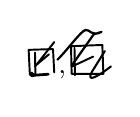
\begin{tikzpicture}[x=.26cm,y=.26cm,line cap=round,line join=round]
\draw[line width=.7pt] (0,0) -- (-.06,1.22) -- (1.13,1.26) -- (1.19,.12);
\draw[line width=1pt] (.06,.1) -- (.2,-.02) -- (.9,.03);
\draw[line width=.7pt] (.25,1.09) -- (.27,.04) .. controls (.19,-.12) and (-.02,-.08) .. (.07,.04);
\draw[line width=.7pt] (.25,.4) -- (1.19,1.6) (.25,.43) -- (.93,1);
\node at (1.58,-.01) {,};
\draw[line width=.7pt] (2.04,.05) -- (2.01,1.4) -- (3.54,1.46) -- (3.59,.05) -- cycle;
\draw[line width=.7pt] (2.18,1.32) -- (2.2,-.02) (2.04,.4) -- (3.09,.89);
\draw[line width=.8pt] (1.35,.74) .. controls (1.86,1.25) and (2.51,2.16) .. (2.72,2.19) .. controls (2.9,2.25) and (3.03,1.84) .. (3.5,2.1) -- (3.12,1.98) -- (2.05,.46);
\draw[line width=.75pt] (3.66,1.16) -- (3.02,.13) .. controls (2.77,-.37) and (3.22,-.15) .. (3.96,.41);
\end{tikzpicture}}
\end{minipage} & \deleted{34}\\
$\left.\begin{array}{@{}l@{}}
\text{aspheric (topos, object of topos, \inserted{map of objects})}\\
\text{locally \uline{aspheric topos, tot.\ asph.\ topos}}
\end{array}\right)$ & 35\\
% The visible opening parenthesis has no matching closing parenthesis.
\uline{Weak equivalence} ($f:X\mathrel{\unsure{-|\to}}Y$ m; of topos & ?\\
homotopy interval & 37\\
{}[strict] elementary modelizer & 39.\\
$\left.\begin{array}{@{}l@{}}
\text{local test catégory}\\
\text{local el.\ modelizer}
\end{array}\right)$ & 39\\
{}[locally] modelizing topos & 39
\end{tabular}}
% archive sheet number: 8

